\documentclass[a4paper,12pt]{article}

\usepackage[14pt]{extsizes}
\usepackage{cmap}					% поиск в PDF
\usepackage{mathtext} 				% русские буквы в формулах
\usepackage[T2A]{fontenc}			% кодировка
\usepackage[utf8]{inputenc}			% кодировка исходного текста
\usepackage[english,russian]{babel}	% локализация и переносы
\usepackage{graphicx}
\usepackage{geometry}
\usepackage{amsmath}
\usepackage[table]{xcolor}
\setlength\extrarowheight{2pt}


\geometry{verbose, a4paper, tmargin=2cm, bmargin=2cm, lmargin=3cm, rmargin=2cm}
\author{Vysotsky Maxim}
\title{Отчёт}
\date{2022}

\begin{document}
	\begin{titlepage}
		\begin{center}
			{Министерство науки и высшего образования Российской Федерации
				НАЦИОНАЛЬНЫЙ ИССЛЕДОВАТЕЛЬСКИЙ ТОМСКИЙ
				ГОСУДАРСТВЕННЫЙ УНИВЕРСИТЕТ (НИ ТГУ)}
		\end{center}
		\begin{center}
			{Физический факультет}
		\end{center}
		
		
		\vspace{8cm}
		{
			\begin{center}
				{\bf Лабораторная работа №30}\\
				Изучение параметрического возбуждения колебаний
			\end{center}
		}
		\vspace{2cm}
		\begin{flushright}
			{Руководитель:\\ канд. физ.-мат. наук\\
				Конов И. А. \\
				Работу выполнили:\\
				Левин Н. Н. \\
				Высоцкий М. Ю.\\
				\vspace{0.2cm}
				гр. 052101}
		\end{flushright}
		\vspace{3cm}
		\begin{center}
			Томск, 2022
		\end{center}
	\end{titlepage}

\section{Теоретическое введение}
\hspace{\parindent}\textbf{Цель работы:} экспериментально исследовать явление параметрического резонанса.

\subsection{Гармонические колебания математического маятника}
Для начала, рассмотрим математический маятник. Если отклонить маятник на угол $\varphi$ из положения равновесия, он начнет совершать вращательное движение вдоль оси $z$, проходящей перендикулярно к плоскости рисунка через точку $O$.

\begin{figure}[h!]
	\begin{center}
		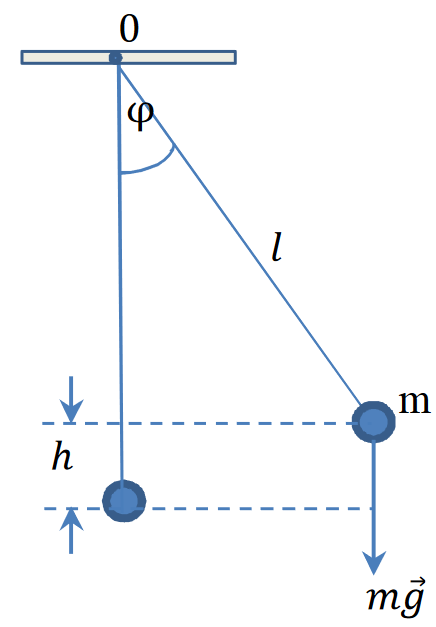
\includegraphics[scale=0.5]{1}
	\end{center}
	\caption{Математический маятник}
\end{figure}

Запишем уравнение динамики вращательного движения относительно оси $z$:
$$\frac{dL_z}{dt} = M_z,$$
где $L_z = I_z\dot\varphi$; $M_z = -mgl\sin\varphi$, если принять за положительное направление $z$, сонаправленное с вектором угловой скорости $\omega$.

Примем массу груза за $m$, длину нити за $l = const$. Тогда мы имеем момент инерции $I_z = ml^2$, который не будет изменяться во время движения. И тогда мы можем записать уравнение в виде:
$$I_z \frac{d^2\varphi}{dt^2} = -mgl\sin\varphi$$

При рассмотрении малых углов, мы можем сказать, что $\sin\varphi \approx \varphi$, и тогда мы получим уравнение:
$$\ddot{\varphi} + \frac{g}{l}\varphi = 0,$$
решением которого будут колебания вида:
$$\varphi = \varphi_0cos(\omega_0t+\alpha),$$
где $\omega_0 = \sqrt{\frac{g}{l}}$ -- собственная частота колебаний математического маятника.

Далее мы рассмотрим изменение полной механической энергии маятника в процессе движения:

Кинетическая энергия равна:
$$E_к = \frac{I(\dot{\varphi})^2}{2} = \frac{1}{2}ml^2\omega_0^2\varphi_0^2[\sin(\omega_0t+\alpha)]^2$$

Потенциальная энергия относительно положения равновесия равна:
$$E_п = mgh = mgl(1-\cos\varphi)$$

Разложив $\cos\varphi$ в ряд Тейлора около точки равновесия маятника $\varphi = 0$, получим $\cos\varphi \approx 1 -\frac{1}{2}\varphi^2$. Тогда мы можем представить потенциальную энергию в виде:
$$E_п = \frac{1}{2}mgl\varphi^2 = \frac{1}{2}\omega_0^2\varphi_0^2[\cos(\omega_0+\alpha)]^2$$
И так как $$\omega_0^2 = \frac{g}{l}$$
$$[\cos(\omega_0+\alpha)]^2 = \frac{1}{2}[1+\cos2(\omega_0+\alpha)]$$
$$[\sin(\omega_0+\alpha)]^2 = \frac{1}{2}[1-\cos2(\omega_0+\alpha)]$$
мы можем представить кинетическую и потенциальную энергию в следующем виде:
$$Е_к = \frac{1}{4}ml^2\omega_0^2\varphi_0^2[1-\cos2(\omega_0+\alpha)]$$
$$Е_п = \frac{1}{4}ml^2\omega_0^2\varphi_0^2[1+\cos2(\omega_0+\alpha)]$$

Следовательно, кинетическая и потенциальная энергии совершают гармонические колебания вокруг общего среднего значения $\frac{1}{4}ml^2\omega_0^2\varphi_0^2$ с удвоенной угловой частотой $2\omega_0$. Полная механическая энергия остается неизменной, и она равна:
$$Е = Е_к + Е_п = \frac{1}{2}ml^2\omega_0^2\varphi_0^2$$

\subsection{Параметрические колебания}
\hspace{\parindent}Параметрическое возбуждение колебаний происходит в результате развития \textbf{параметрической неустойчивости}, возникающей при периодическом воздействии на те параметры системы, которые определяют величину запасённой колебательной энергии. Для математического маятника – это длина нити или масса груза.

Пусть длина нити изменяется со временем. Мы имеем зависимость $l = l(t)$. Тогда
$$\frac{d(ml^2\dot{\varphi})}{dt} = -mgl\sin\varphi$$
примет вид
$$2ml\dot l\dot\varphi + ml^2\ddot{\varphi} +mgl\sin\varphi=0$$

Для малых углов отклонения маятника из положения равновесия получим уравнение вида:

$$\ddot{\varphi} + \frac{2\dot{l}}{l}\dot{\varphi} + \frac{g}{l}\varphi = 0$$

В методическом пособии указано, что "анализ и решение данного уравнения очень сложны", потому они опускаются. Также нужно учитывать, что данное уравнение получается для малых углов, не превышающих значения $\varphi_{пред.} \approx 8^{\circ}$. В случае б\'{о}льших отклонений появляются нелинейные эффекты, когда период собственных колебаний начинает зависеть от амплитуды колебаний $\varphi_0$.

\begin{equation}
T_{0 нел.}\varphi_0 \approx T_0(1+ \frac{\varphi_0^2}{16})
\end{equation}











\end{document}